\documentclass[12pt]{report}

\usepackage{tikz}
\usepackage[utf8]{inputenc}
\usepackage[T1]{fontenc}

% Core math & theorem environments
\usepackage{amsmath,amsfonts,amssymb,amsthm}
\usepackage{bm}
\newtheorem{lemma}{Lemma}[section]
\newtheorem{proposition}[lemma]{Proposition}
\newtheorem{theorem}{Theorem}
\usetikzlibrary{decorations.pathreplacing,arrows.meta,calc}
% Better tables
\usepackage{booktabs}

% Floating objects
\usepackage{float}

% Algorithms
\usepackage{algorithm}
\usepackage{algpseudocode}
\usepackage{thmtools}
% Graphics & captions (if you add figures later)
\usepackage{graphicx}

% \usepackage{graphics}
\usepackage{caption}
\usepackage{subcaption}


\graphicspath {{figs/}}
\newcommand{\incfig}[1]{%
		\def\svgwidth{\columnwidth}
		\import{./figs/}{#1.png}
	}
% Cross‐references
\usepackage{hyperref}
\usepackage{cleveref}
\usepackage[top=2cm, bottom=2cm, left=2cm, right=2cm]{geometry}
\geometry{a4paper}
\usepackage{fancyhdr}
\renewcommand{\headrulewidth}{0pt}
\renewcommand{\contentsname}{Table of Contents}
\setlength{\parindent}{0pt}
\date{}
\pagestyle{fancyplain}
\begin{document}
\begin{titlepage}
	Tskip0pt
	\centering
	\vspace*{\fill}
	{\bf \LARGE BFGS : An Optimzation Algorithm\\}
	\vspace{1cm}
	{\Large University of California, Merced\\}
	\vspace{0.5cm}
	{\large Department of Applied Mathematics\\}
	\vspace{1.5cm}
	{\bf \Large Math 231 Final Project Report\\}
	\vspace{1.5cm}
	{\bf \Large Pratham Lalwani\\}
	\vspace{2cm}
	{\large May 13, 2025\\}
	\vspace*{\fill}
\end{titlepage}

\clearpage
\setcounter{page}{1}
\renewcommand{\thepage}{\roman{page}}

%\chapter*{Declaration}
%\addcontentsline{toc}{chapter}{Declaration}
%
%\emph{\hskip -2mm \begin{tabular}{p{6cm}} I, \hrulefill , \\\end{tabular} declare the proposed project work is based on my original work, except on ideas or data within acknowledged citations. I declare the proposed work is carried out solely by myself and has not been submitted previously or concurrently for any other course or degree from UNBC or other institutes.}

\chapter*{Abstract}
\addcontentsline{toc}{chapter}{Abstract}
Optimizing functions is a very important problem which has applications across disciplines from Mathematics and Science to Finance. In cases where analytical solution doesn't exist to a problem we have to rely on optimization algorithms to find a minimum or maximum of the given function. First order methods like gradient descent although cheap are very slow at converging to a minima whereas Newton's method is quite expensive. Quasi-Newton like BFGS provide middle ground and allow a "Newton like" update without having to find the Hessian.

\tableofcontents
\addcontentsline{toc}{chapter}{Table of Contents}
\newpage
\listoffigures
\addcontentsline{toc}{chapter}{List of Figures}
\newpage
\listoftables
\addcontentsline{toc}{chapter}{List of Tables}
\newpage
\renewcommand{\thepage}{\arabic{page}}
\setcounter{page}{1}

% -------------------------
% Chapter 1: Introduction
% -------------------------
\chapter{Introduction}
Optimization problems are ubiquitous. From solving linear problems to large-scale physical simulations, minimizing a function is required. Due to the wide range of optimization problems available, a good optimization algorithm is general, makes minimal assumptions, and is fast. One such algorithm is BFGS (named after Broyden, Fletcher, Goldfarb, and Shanno), which provides superlinear convergence.

BFGS is one of the most widely used algorithms for optimization. It works by approximating the Hessian of the objective function, which we want to minimize and applying symmetric updates such that its inverse of the Hessian can be computed in $\mathcal{O}(n^2)$ operations. Compared to Newton's method, which usually has a dense linear system to solve, requiring $\mathcal O(n^3)$ operations to solve.

Even though BFGS is more efficient than Newton's method, the $ \mathcal O(n^2)$ cost per iteration is high. To maximize each iteration, we perform a line search along a proposed search direction to minimize the function along the search direction.

In this report we will discuss the Wolfe conditions to terminate a line search, the BFGS update, the convergence of Quasi Newton methods and their rate of convergence.
% -------------------------

% Chapter 2: Main Results
% -------------------------
\chapter{Main Results}

\section{Background}
We consider the unconstrained optimization problem
\[
	\min_{x\in\mathbb{R}^n} f(x),
\]
where $f:\mathbb{R}^n\to\mathbb{R}$ is twice continuously differentiable and bounded below.
A line‐search method generates iterates
\begin{equation}
	\bm x_{k+1} = \bm x_k + \alpha_k \bm p_k, \label{eq:opt_update}
\end{equation}
where $p_k$ is a search direction (e.g.\ a quasi‐Newton direction) and $\alpha_k>0$ is called the step size chosen to satisfy the \emph{Wolfe conditions}:
\begin{align}
	f(\bm x_k + \alpha \bm p_k)                  & \le f(x_k) + c_1 \alpha \nabla f(x_k)^T p_k, \label{eq:sufficient-decrease} \\
	\nabla f(\bm x_k + \alpha \bm p_k)^T \bm p_k & \ge c_2 \nabla f(x_k)^T \bm p_k \label{eq:curvature-condition},
\end{align}
with constants $0 < c_1 < c_2 < 1$.
$\ref{eq:sufficient-decrease}$ is called the sufficient decrease condition, which checks for decrease of the objective function along the descent direction and \ref{eq:curvature-condition} only allows for a smaller directional derivative along the descent direction is called the curvature condition.

\begin{figure}[htpb]
	\centering
	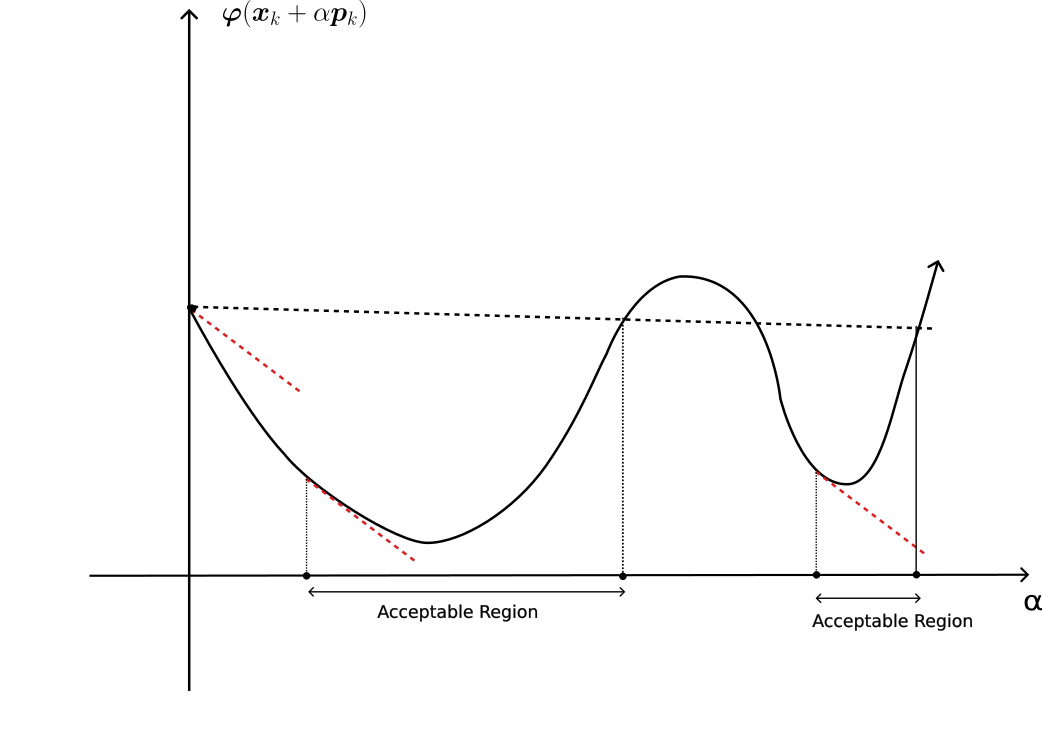
\includegraphics[width=0.7\textwidth]{./drawing.png}
	\caption{Acceptable regions for the Wolfe conditions}
	\label{fig:Wolfe}
\end{figure}
The existence of such and $\alpha$ is guaranteed by the theorem below:
\begin{lemma}
	Suppose $f: \mathbb{R}^n \rightarrow \mathbb{R}$ is continuously differentiable. Let $\bm p_k$ be a descent direction at $\bm x_k$, and assume that $f$ is bounded below along the ray $\left\{\bm x_k+\alpha \bm p_k \mid \alpha>0\right\}$. Then if $0<c_1<$ $c_2<1$, there exist intervals of step size the Wolfe conditions \eqref{eq:sufficient-decrease} and \eqref{eq:curvature-condition}.
\end{lemma}
A good value of $c_1 = 10^{-4}$ and $c_2 = 0.9$.\cite{nocedal}

Now we shall find a good $\bm p_k$. The best search direction is given by Newton's update, which is $\bm p_k = -(\nabla^2f)^{-1}(\bm x_k)\nabla f(\bm x_k)$. Quasi-Newton methods usually construct an approximation $B_k \approx \nabla^2 f(\bm x_k)^{-1}$ to provide a search direction,
\begin{equation}
	\bm p_k = -B_k^{-1}\nabla f(\bm x_k) \label{eq:QNupd}
\end{equation}
One such Quasi Newton method is the BFGS (Broyden, Fletcher, Goldfarb and Shanno) algorithm. BFGS directly constructs the inverse Hessian as follows:
\[
	H_{k+1}=H_k+\frac{\left(\bm{s}_k^{\mathrm{T}} \bm{y}_k+\bm{y}_k^{\mathrm{T}} H_k \bm{y}_k\right)\left(\bm{s}_k \bm{s}_k^{\mathrm{T}}\right)}{\left(\bm{s}_k^{\mathrm{T}} \bm{y}_k\right)^2}-\frac{H_k \bm{y}_k \bm{s}_k^{\mathrm{T}}+\bm{s}_k \bm{y}_k^{\mathrm{T}} H_k}{\bm{s}_k^{\mathrm{T}} \bm{y}_k}
	.\]
Where $H_k \approx (\nabla^2f)^{-1}(\bm x_k)$.
For convenience, we define $f(\bm x_k) := f_k$.
We shall now prove the convergence and rate of convergence of BFGS. To prove the result, we need the following lemmas:
\begin{lemma}[Taylor's Theorem]
	Suppose that $f: \mathbb{R}^n \rightarrow \mathbb{R}$ is continuously differentiable and that $p \in \mathbb{R}^n$. Then we have,

	\[
		f(\bm x+\bm p)=f(\bm x)+\nabla f(\bm x+t \bm p)^T \bm p
	\]

	for some $t \in(0,1)$. Moreover, if $f$ is twice continuously differentiable, we have that

	\[
		\nabla f(\bm x+\bm p)=\nabla f(\bm x)+\int_0^1 \nabla^2 f(\bm x+t \bm p) \bm p d t
	\]

	and that

	\[
		f(\bm x+\bm p)=f(\bm x)+\nabla f(\bm x)^T \bm p+\frac{1}{2} \bm p^T \nabla^2 f(\bm x+t \bm p) \bm p
	\]

	for some $t \in(0,1)$.
\end{lemma}
\begin{lemma}
	Suppose that $f: \mathbf{R}^n \rightarrow \mathbf{R}$ is twice continuously differentiable. Consider the iteration $\bm x_{k+1}=\bm x_k+\alpha_k \bm p_k$, where $\bm p_k$ is a descent direction and $\alpha_k$ satisfies the Wolfe conditions with $c_1 \leq 1 / 2$. If the sequence $\left\{\bm x_k\right\}$ converges to a point $\bm x^*$ such that $\nabla f\left(\bm x^*\right)=0$ and $\nabla^2 f\left(\bm x^*\right)$ is positive definite, and if the search direction satisfies
	\begin{equation}
		\lim _{k \rightarrow \infty} \frac{\left\|\nabla f_k+\nabla^2 f_k \bm p_k\right\|}{\left\|\bm p_k\right\|}=0  \label{eq:gcond}
	\end{equation}
	then
	\begin{itemize}
		\item the step length $\alpha_k=1$ is admissible for all $k$ greater than a certain index $k_0$; and
		\item if $\alpha_k=1$ for all $k>k_0,\left\{x_k\right\}$ converges to $x^*$ superlinearly.
	\end{itemize}
\end{lemma}
We also define the following quantity,
\begin{equation}
	\cos(\theta_k) =- \frac{p_k^{T}\nabla f(\bm x_k)}{\|\bm p_k\| \|\nabla f_k\|}
\end{equation}
which measures the deviation between the gradient and the descent direction.
\begin{theorem}
	\label{thm:thm1}
	Consider any iteration of the form \eqref{eq:opt_update}, where $\bm p_k$ is a descent direction and $\alpha_k$ satisfies the Wolfe conditions. Suppose that $f$ is bounded below in $\mathbb{R}^n$ and that $f$ is continuously differentiable in an open set $\mathcal{M}$ containing the level set $\mathcal{L} \stackrel{\text { def }}{=}\left\{\bm x: f(\bm x) \leq f\left(\bm x_0\right)\right\}$, where $\bm x_0$ is the starting point of the iteration. Assume also that the gradient $\nabla f$ is Lipschitz continuous on $\mathcal{N}$, that is, there exists a constant $L>0$ such that
	\begin{equation}
		\|\nabla f(\bm x)-\nabla f(\tilde{\bm x})\| \leq L\|\bm x-\tilde{\bm x}\|, \quad \text { for all } \bm x, \tilde{\bm x} \in \mathcal{N} .
	\end{equation}
	Then

	\begin{equation}
		\sum_{k \geq 0} \cos ^2 \theta_k\left\|\nabla f_k\right\|^2<\infty \label{eq:cos_conv}
	\end{equation}
\end{theorem}
it can be shown that the condition $\eqref{eq:gcond}$ is equivalent to the following,
\begin{equation}
	\lim_{k \to \infty} \frac{\|(B_{k} - \nabla^2f(x^{*}))p_k \|}{\|p_k\|} = 0 \label{eq:QN_matcond}
\end{equation}
\begin{theorem}
	\label{thm:thm2}
	Suppose that $f: \mathbb{R}^n \rightarrow \mathbb{R}$ is twice continuously differentiable. Consider the iteration $x_{k+1}=x_k+p_k$ (that is, the step length $\alpha_k$ is uniformly 1 ) and that $p_k$ is given by \eqref{eq:QNupd} Let us assume also that $\left\{x_k\right\}$ converges to a point $x^*$ such that $\nabla f\left(x^*\right)=0$ and $\nabla^2 f\left(x^*\right)$ is positive definite. Then $\left\{x_k\right\}$ converges superlinearly if and only if $\eqref{eq:QN_matcond}$ holds.
\end{theorem}
\section{Theoretical Results}
\subsection{Convergence of Quasi Newton}
\begin{proof}[Proof of \autoref{thm:thm1}]
	From the curvature condition \eqref{eq:curvature-condition} and the update \eqref{eq:opt_update} we have
	\[
		(\nabla f_{k+1}-\nabla f_k)^T p_k \;\ge\;(c_2-1)\,\nabla f_k^T p_k,
	\]
	while the Lipschitz condition \eqref{eq:sufficient-decrease} implies
	\[
		(\nabla f_{k+1}-\nabla f_k)^T p_k \le L \|\bm x_{k}-\alpha_k \bm p_k -\bm x_{k}\| \|p_k\| \le\alpha_k\,L\,\|p_k\|^2.
	\]
	Combining these two inequalities gives
	\[
		\alpha_k \;\ge\;\frac{c_2-1}{L}\;\frac{\nabla f_k^T p_k}{\|p_k\|^2}.
	\]
	Substituting this bound into the sufficient-decrease condition \eqref{eq:sufficient-decrease} yields
	\[
		f_{k+1}
		\;\le\;
		f_k - c_1\,\alpha_k\,\nabla f_k^T p_k
		\;\le\;
		f_k - c_1\frac{1-c_2}{L}\,\frac{(\nabla f_k^T p_k)^2}{\|p_k\|^2}.
	\]
	From \eqref{eq:cos_conv}, this becomes
	\[
		f_{k+1} \;\le\; f_k \;-\; c\,\cos^2\theta_k\,\|\nabla f_k\|^2,
	\]
	where $c = c_1(1-c_2)/L$.  Using the recursive relation gives
	\begin{equation}\label{eq:3.15}
		f_{k+1} \;\le\; f_0 \;-\; c\sum_{j=0}^k \cos^2\theta_j\,\|\nabla f_j\|^2.
	\end{equation}
	Since $f$ is bounded below, the left‐hand side of \eqref{eq:3.15} remains finite as $k\to\infty$.  Hence
	\[
		\sum_{k=0}^\infty \cos^2\theta_k\,\|\nabla f_k\|^2 < \infty,
	\]
	which is the desired result.
\end{proof}
If we can show that $\cos^2(\theta_k) > m>0$ then we shall have $\|\nabla f_k\| \to 0$
Suppose we have a Quasi Newton update matrix $B_k$ which is positive definite and has a bounded condition number.
It is easy to show that for any non-singular matrix A, we have the relation,
\[
	\frac{\|\bm x\|}{\|A^{-1}\|} = \|A\bm x\|
	.\]
So we have,
\[
	\frac{\|\bm x\|}{\|B^{-1}\|} = \|B\bm x\|
	.\]
Consider,
\begin{align*}
	\cos(\theta_k) & =   -\frac{\bm p_k \nabla f(\bm x_k)}{\|\bm p_k\|\|\nabla f(\bm x_k) \|} \\
	               & =   \frac{\bm p_k B_k \bm p_k }{\|\bm p_k\|\|B_k \bm p_k \|} \\
	               & \ge \frac{\|\bm p_k\|^2}{\|B_k^{-1}\| \|B_k\| \|\bm p_k\|^2} \\
	               & \ge \frac{1}{\kappa(B_k)}
	.\end{align*}
Therefore, for a Quasi Newton we have the result,
\[
	\lim_{k \to \infty} \|\nabla f(\bm x_k)\| = 0
	.\]
Which means the BFGS iteration converges given a bounded condition number.
\begin{proof}[Proof of \autoref{thm:thm2}]
	We define the Newton Descent direction as follows,
	\[
		\bm p_k^{N} = (\nabla^2f)^{-1} \nabla f(\bm x_k)
		.\]
	We first show that it is equivalent to \eqref{eq:QN_matcond}
	\begin{equation}
		\bm p_k-\bm p_k^{\mathrm{N}}=o\left(\left\|\bm p_k\right\|\right) \label{eq:dir_eq}.
	\end{equation}
	Suppose \eqref{eq:QN_matcond} holds for $B_k$,

	\[
		\begin{aligned}
			\bm p_k-\bm p_k^{\mathrm{N}} & =\nabla^2 f_k^{-1}\left(\nabla^2 f_k \bm p_k+\nabla f_k\right)               \\
			                             & =\nabla^2 f_k^{-1}\left(\nabla^2 f_k-B_k\right) \bm p_k                      \\
			                             & =\mathcal O\left(\left\|\left(\nabla^2 f_k-B_k\right) \bm p_k\right\|\right) \\
			                             & = o\left(\left\|\bm p_k\right\|\right).
		\end{aligned}
	\]
	Now we suppose \eqref{eq:dir_eq} is true,
	\begin{align*}
		\bm p_k-\bm p_k^{\mathrm{N}}                     & = o(\|\bm p_k\|) \\
		\nabla^2f(\bm x_k)(\bm p_k-\bm p_k^{\mathrm{N}}) & = o(\|\nabla f^2(\bm x_k)\|\|\bm p_k\|)
		.\end{align*}
	As we have a bounded hessian near $x^{*}$, therefore, for sufficiently large $x_k$ we get,
	\begin{align*}
		\nabla^2f(\bm x_k)(\bm p_k-\bm p_k^{\mathrm{N}})                  & = o(\|\bm p_k\|) \\
		\nabla^2f(\bm x_k)\bm p_k- \nabla^2f(\bm x_k)\bm p_k^{\mathrm{N}} & = o(\|\bm p_k\|) \\
		\nabla^2f(\bm x_k)\bm p_k- \nabla f(\bm x_k)                      & = o(\|\bm p_k\|) \\
		\nabla^2f(\bm x_k)\bm p_k- B_k^{-1}\bm p_k                        & = o(\|\bm p_k\|)
		.\end{align*}
	Which is the same as \eqref{eq:QN_matcond}.

	By combining (3.33) and (3.37), we obtain that

	\[
		\left\|\bm x_k+\bm p_k-\bm x^*\right\| \leq\left\|\bm x_k+\bm p_k^{\mathrm{N}}-\bm x^*\right\|+\left\|\bm p_k-\bm p_k^{\mathrm{N}}\right\|=O\left(\left\|\bm x_k-\bm x^*\right\|^2\right)+o\left(\left\|\bm p_k\right\|\right) .
	\]
	Now we bound $\|\bm p_k\|$,
	\begin{align*}
		\|\bm p_k\| & = \|\bm x_k +\bm p_k - \bm x^{*} -\left(\bm x_{k} - \bm x^{*}  \right) \| \\
		            & \le \|\bm x_k +\bm p_k - \bm x^{*} \|+\|\bm x_{k} - \bm x^{*}   \| \\
		            & \le \|\bm x_{k} - \bm x^{*} \| +O\left(\left\|\bm x_k-\bm x^*\right\|^2\right)+o\left(\left\|\bm p_k\right\|\right) \\
		            & = O\left( \|\bm x_{k} - \bm x^{*} \|\right)
		.\end{align*}
	Therefore,
	\[
		\left\|\bm x_k+\bm p_k-\bm x^*\right\| \leq o\left(\left\|\bm x_k-\bm x^*\right\|\right),
	\]
	which gives,
	\[\left\|\bm x_{k+1}-\bm x^*\right\| \leq o\left(\left\|\bm x_k-\bm x^*\right\|\right)\]
	giving the superlinear convergence result.
\end{proof}
We shall now derive the Inverse Hessian update of BFGS.
\subsubsection{BFGS Update Derivation}
We would like to update the Hessian such that we have to make small updates to the matrix.\\
\begin{gather*}
	\min \| H-H_{k}\|_W^{2}\quad  H \in \mathbb{R}^{n \times n} \quad \text{subject to constraint,} \\
	H \bm y_{k}=\bm{s}_k \quad \text { and } H^{T}=H
	.\end{gather*}


The norm is the weighted Frobenius norm, and $W$ is a symmetric Positive Definite matrix.

As $W$ is SPD we have a matrix $W^{1/2}$ such that:\\
$$
	W^{1 / 2} W^{1 / 2}=W
$$

Therefore, the weighted Frobenius norm is,

$$
	\begin{aligned}
		\left\|H-H_{k}\right\|_{W}^{2} & =\left\|W^{1 / 2}\left(H-H_{k}\right) W^{1 / 2}\right\|_{ F}^{2} \\
	\end{aligned}
$$

We define the Lagrange Multiplier Problem as follows:

\begin{align}
	 & \mathcal L(H, \lambda, \theta)=\left\|H-H_{k}\right\|_{W}^{2}+\operatorname{tr}\left(\lambda^{T}\left(H y_{k}-\bm{s}_k\right)\right) +\left(H^{T}-H\right) \Theta
\end{align}
Taking the respective partials,
\begin{align}
	 & \frac{\partial\mathcal L}{\partial \bm{\lambda}}=H \bm{y}_k-\bm{s}_{k}=0\nonumber \\
	 & \frac{\partial\mathcal L}{\partial \Theta}= O \implies H^{T}=H\nonumber \\
	 & \frac{\partial\mathcal L}{\partial H}=W\left(H-H_{k}\right) W+\bm{\lambda} \bm{y}_k^{T}+\Theta-\Theta^{T}=0\nonumber \\
	 & \therefore W H_{W} W=W H_{k} W+ \bm{\lambda} \bm{y}_k^{T}+\Theta-\Theta^{T}\label{eq:equation1}
	.\end{align}
Applying the transpose on both sides
\begin{equation}
	W H_{k} W=W H_{k} W+\bm{y}_k^{T} \bm{\lambda}^{T}-\left(\Theta-\Theta^{T}\right) \label{eq:equation2}
\end{equation}

Subtracting \eqref{eq:equation2} from \eqref{eq:equation1} :
\begin{align}
	 & 0=\left(\bm \lambda  \bm{y}_k^{T}- \bm y_{k} \bm \lambda^{T}\right)+2\left(\Theta-\Theta^{T}\right)\nonumber \\
	 & \frac{1}{2}\left(\bm y_{k} \bm \lambda^{T}-\bm \lambda \bm y_{k}^{T}\right)=\Theta-\Theta^{T} \label{eq:eq3}
\end{align}
Using \eqref{eq:eq3} in \eqref{eq:equation1}
\begin{align*}
	W H_{k} W=W H_{k} W+\frac{1}{2}\left(\bm{\lambda} y_{k}^{T}+y_{k} \bm{\lambda}^{T}\right) \\
	.\end{align*}
$$
	H_{k}=H_{k}+\frac{1}{2} W^{-1}\left(\bm{\lambda}_{\bm{\lambda}} \bm{y}_k^{T}+\bm{y}_{k} \bm \lambda^{T}\right) W^{-1}
$$

We also have

$$
	H{\bm{y}_k}=\bm{s}_{k}
$$


We also didn't choose a specific matrix $W$, one good choice is $W \bm{s}_{k}=\bm{y}_k$. Which results in the BFGS update formula.


$$
	\begin{aligned}
		 & H_{k} \bm{y}_k+\frac{1}{2} W^{-1}\left(\bm{\lambda} \bm{y}_{k}^{T}+\bm{y}_{k} \bm{\lambda}^{T}\right) W^{-1} \bm{y}_{k}=\bm{s}_{k}                           \\
		 & H_{k} \bm{y}_k+\frac{1}{2} W^{-1} \bm{\lambda} \bm{y}_{k}^{T} W^{-1} \bm{y}_{k}+\frac{1}{2} W^{-1} \bm{y}_{k} \bm{\lambda}^{T} W^{-1} \bm{y}_{k} =\bm{s}_{k}
	\end{aligned}
$$

$$
	\begin{aligned}
		 & W H_{k} \bm{s}_{k}+\frac{1}{2}\left(\bm{\lambda} \bm{y}_k^{T}+\bm{y}_{k}^{T} \bm{\lambda}^{T}\right) W^{-1} \bm{y}_{k}=W \bm{s}_{k}                           \\
		 & \quad \frac{1}{2}\left(\bm{\lambda} \bm{y}_k W^{-1} \bm{y}_{k}+\bm{y}_{k} \bm{\lambda}^{T} W^{-1} \bm{y}_{k}\right)=W\left(\bm{s}_{k}-H_{k} \bm{y_{k}}\right) \\
		 & \bm{\lambda}=\frac{2 W\left(\bm{s}_{k}-H_{k} \bm{y}_k\right)-\bm{y}_{k} \bm{\lambda}^{T} W^{-1} \bm{y}_{k}}{\bm{y}_{k} W^{-1} {\bm y_{k}}}
	\end{aligned}
$$
Multiplying both sides by $\bm{y}_k^{T} W^{-1}$ and applying transpose.
$$
	\begin{aligned}
		\bm{\lambda}^{T} W^{-1} \bm{y}_k & =
		\left(\frac{2(\bm{y}_{k}^{T} \bm{s}_k
		-\bm y_{k}^{T}H_k \bm y_{k})
		- \left(\bm{y}_{k}^{T} W^{-1} \bm{y}_{k}\right)
		\left(\bm{\lambda}^{T} W^{-1} \bm{y}_{k}\right)}{\bm{y}_k^{T} W^{-1} y_{k}                                                                                                          }\right) \\
		\bm{\lambda}^{T} W^{-1} \bm{y}_k & =
		\frac{\bm{y}_{k}^{T} \bm{s}_k
		-\bm y_{k}^{T}H_k \bm y_{k}
		}{\bm{y}_k^{T} W^{-1} y_{k}}
	\end{aligned}
$$

$$
	\begin{aligned}
		\therefore \bm{\lambda}  & =\frac{2 W\left(\bm{s}_{k}-H_{k} \bm{y}_k\right)}{\bm{y}_{k}^{T} W^{-1} \bm{y}_{k}}-\frac{\bm{y}_{k}\left(\bm y_{k}^{T} {\bm s}_{k} - \bm{y}_{k}^{T} H_{k} \bm{y}_{k} \right)}{\left(\bm{y}_{k}^{T} W^{-1} \bm{y}_{k}\right)^{2}}                                                                    \\
		\text { with } W\bm{s}_k & = \bm y_{k} \implies {\bm s_{k}}=W^{-1} \bm{y}_k                                                                                                                                                                                                                                                     \\
		\bm{\lambda}             & =\frac{2 W\left({\bm{s}_k}-H_{k} \bm{y}_k\right)}{\bm y_{k}^{T}\bm s_{k}}-\frac{\bm{y}_{k}\left(\bm y_{k}^{T} \bm s_{k}-\bm{y}_{k}^{T} H_{k} \bm{y}_{k}\right)}{\left(\bm y_{k}^{T} \bm s_{k}\right)^{2}}                                                                                            \\
		H                        & =  H_{k}+\frac{1}{2} W^{-1} \left(\left(\frac{2 W\left(\bm{s}_k-H_{k} \bm{y}_k\right)}{\bm y_{k}^{T} \bm s_{k}}\right) \bm y_{k}^{T}- \bm{y}_{k}\bm{y}_k^{T}\frac{\left(\bm y_{k}^{T} \bm s_{k}-\bm y_{k}^{T} H_{k} \bm y_{k}\right)}{\left(\bm y_{k}^{T}\bm s_{k}\right)^{2}}               \right. \\
		                         & \left.+\frac{2 \bm y_{k}\left(\bm{s}_k-H_{k} \bm y_{k}\right)^{T} W}{\bm y_{k}^{T} \bm s_{k}}-\bm{y}_k \bm{y}_{k}^{T}\left(\frac{\bm{y}_{k}^{T} \bm s_{k}-\bm{y}_{k}^{T} H_{k} \bm{y}_{k}}{\left(\bm{y}_{k}^{T} \bm{s}_{k}\right)^{2}}\right)\right){W^{-1}}                                         \\
		                         & H=H_{k}+ \frac{\left(\bm{s}_k-H_{k} \bm{y}_k\right) \bm{s}_{k}^{T}}{\bm{y}_{k}^{T} \bm s_{k}}-\frac{\bm s_{k} \bm s_{k}^{T}\left(\bm y_{k}^{T} \bm s_{k}-\bm y_{k}^{T} H_{k} \bm y_{k}\right)}{\left(\bm y_{k}^{T}  \bm s_{k}\right)^{2}}
		+\frac{\bm{s}_k\left(\bm s_{k}-H_{k} \bm y_{k}\right)^{T}}{\bm y_{k}^{T} \bm s_{k}}
	\end{aligned}
$$
We leave it here because this is the efficient way to compute it.


\section{Numerical Results}
\subsection{Examples}
\subsubsection{Rosenbrock Function}
\begin{figure*}[htpb]
	\centering
	\begin{subfigure}[t]{0.4\textwidth}
		\centering
		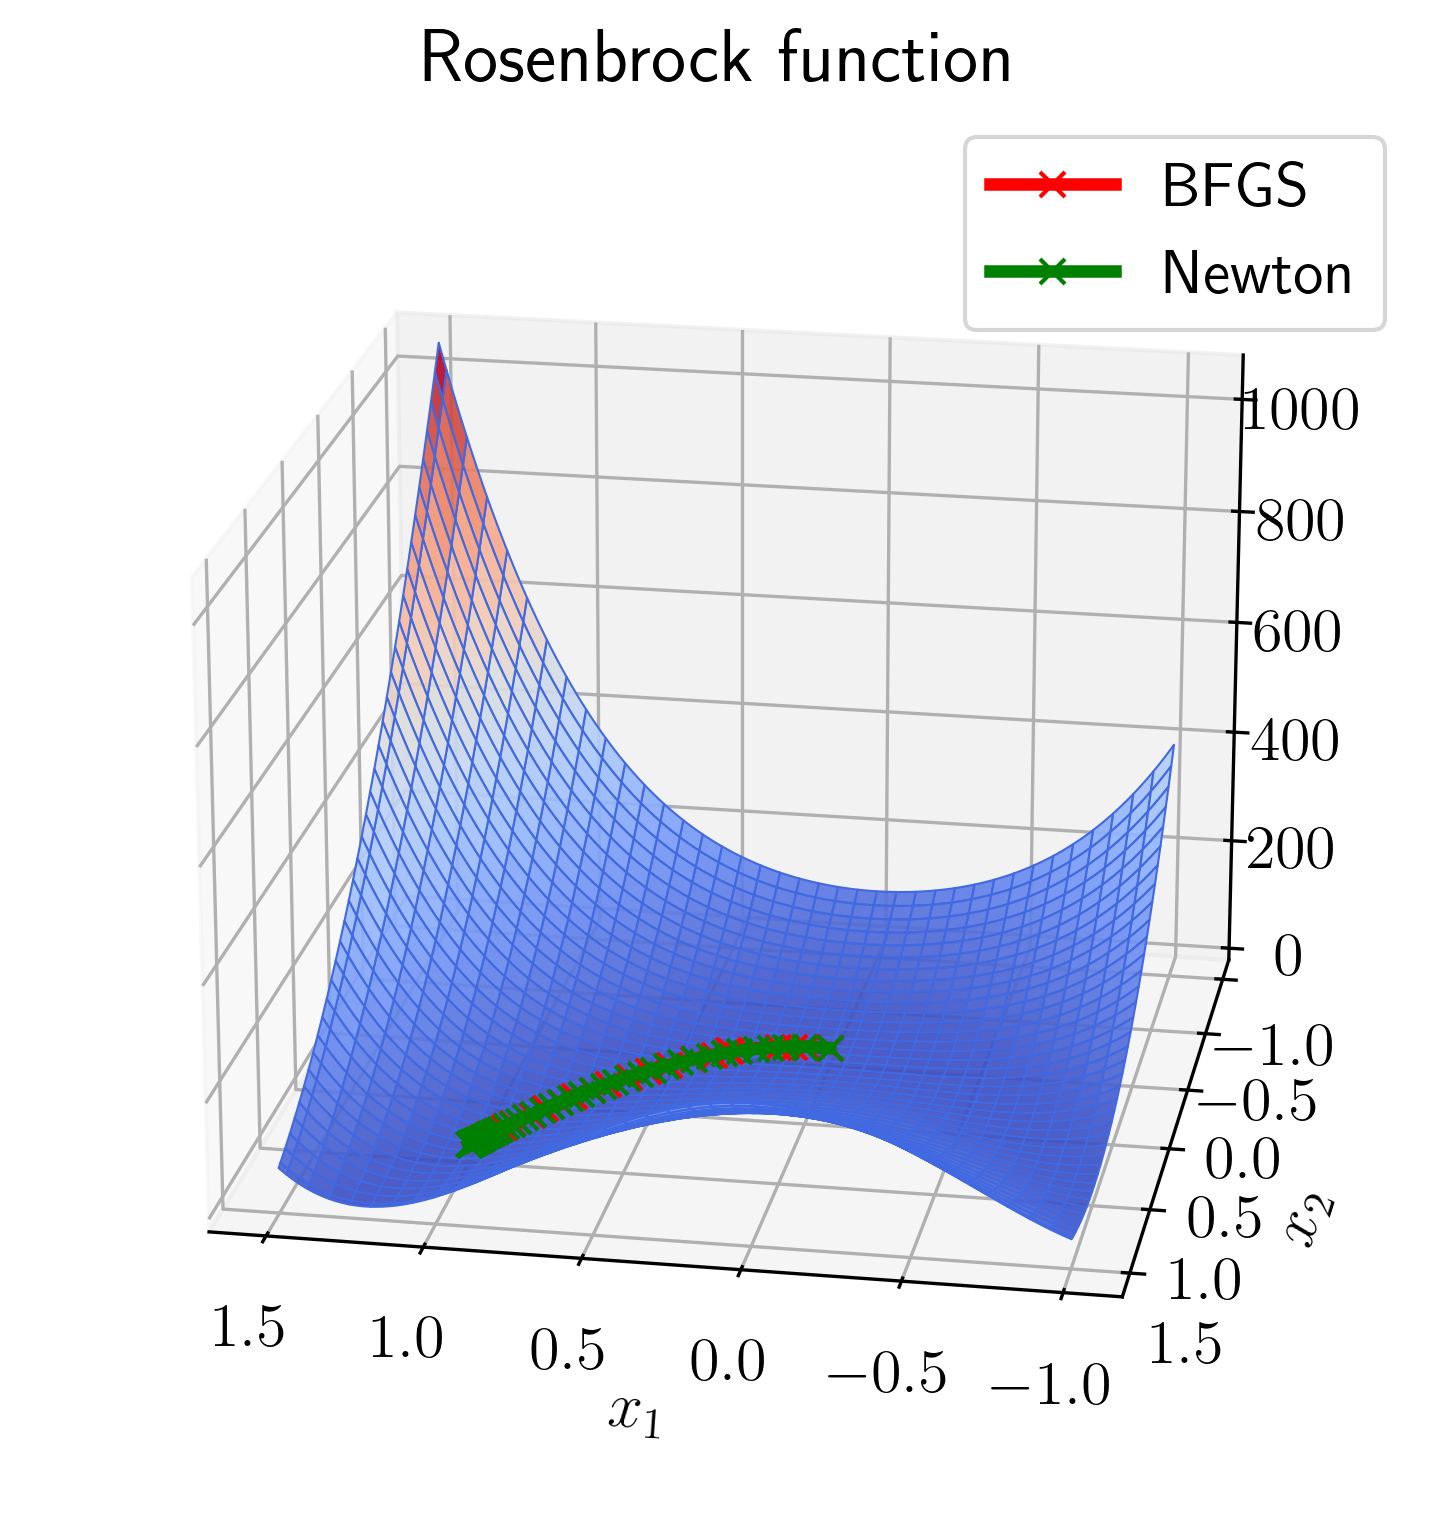
\includegraphics[width=\textwidth]{figs/rosenbrock_surface.png}
		% \caption{BFGS and Newton applied on the Rosenbrock function}
	\end{subfigure}
	\begin{subfigure}[t]{0.4\textwidth}
		\centering
		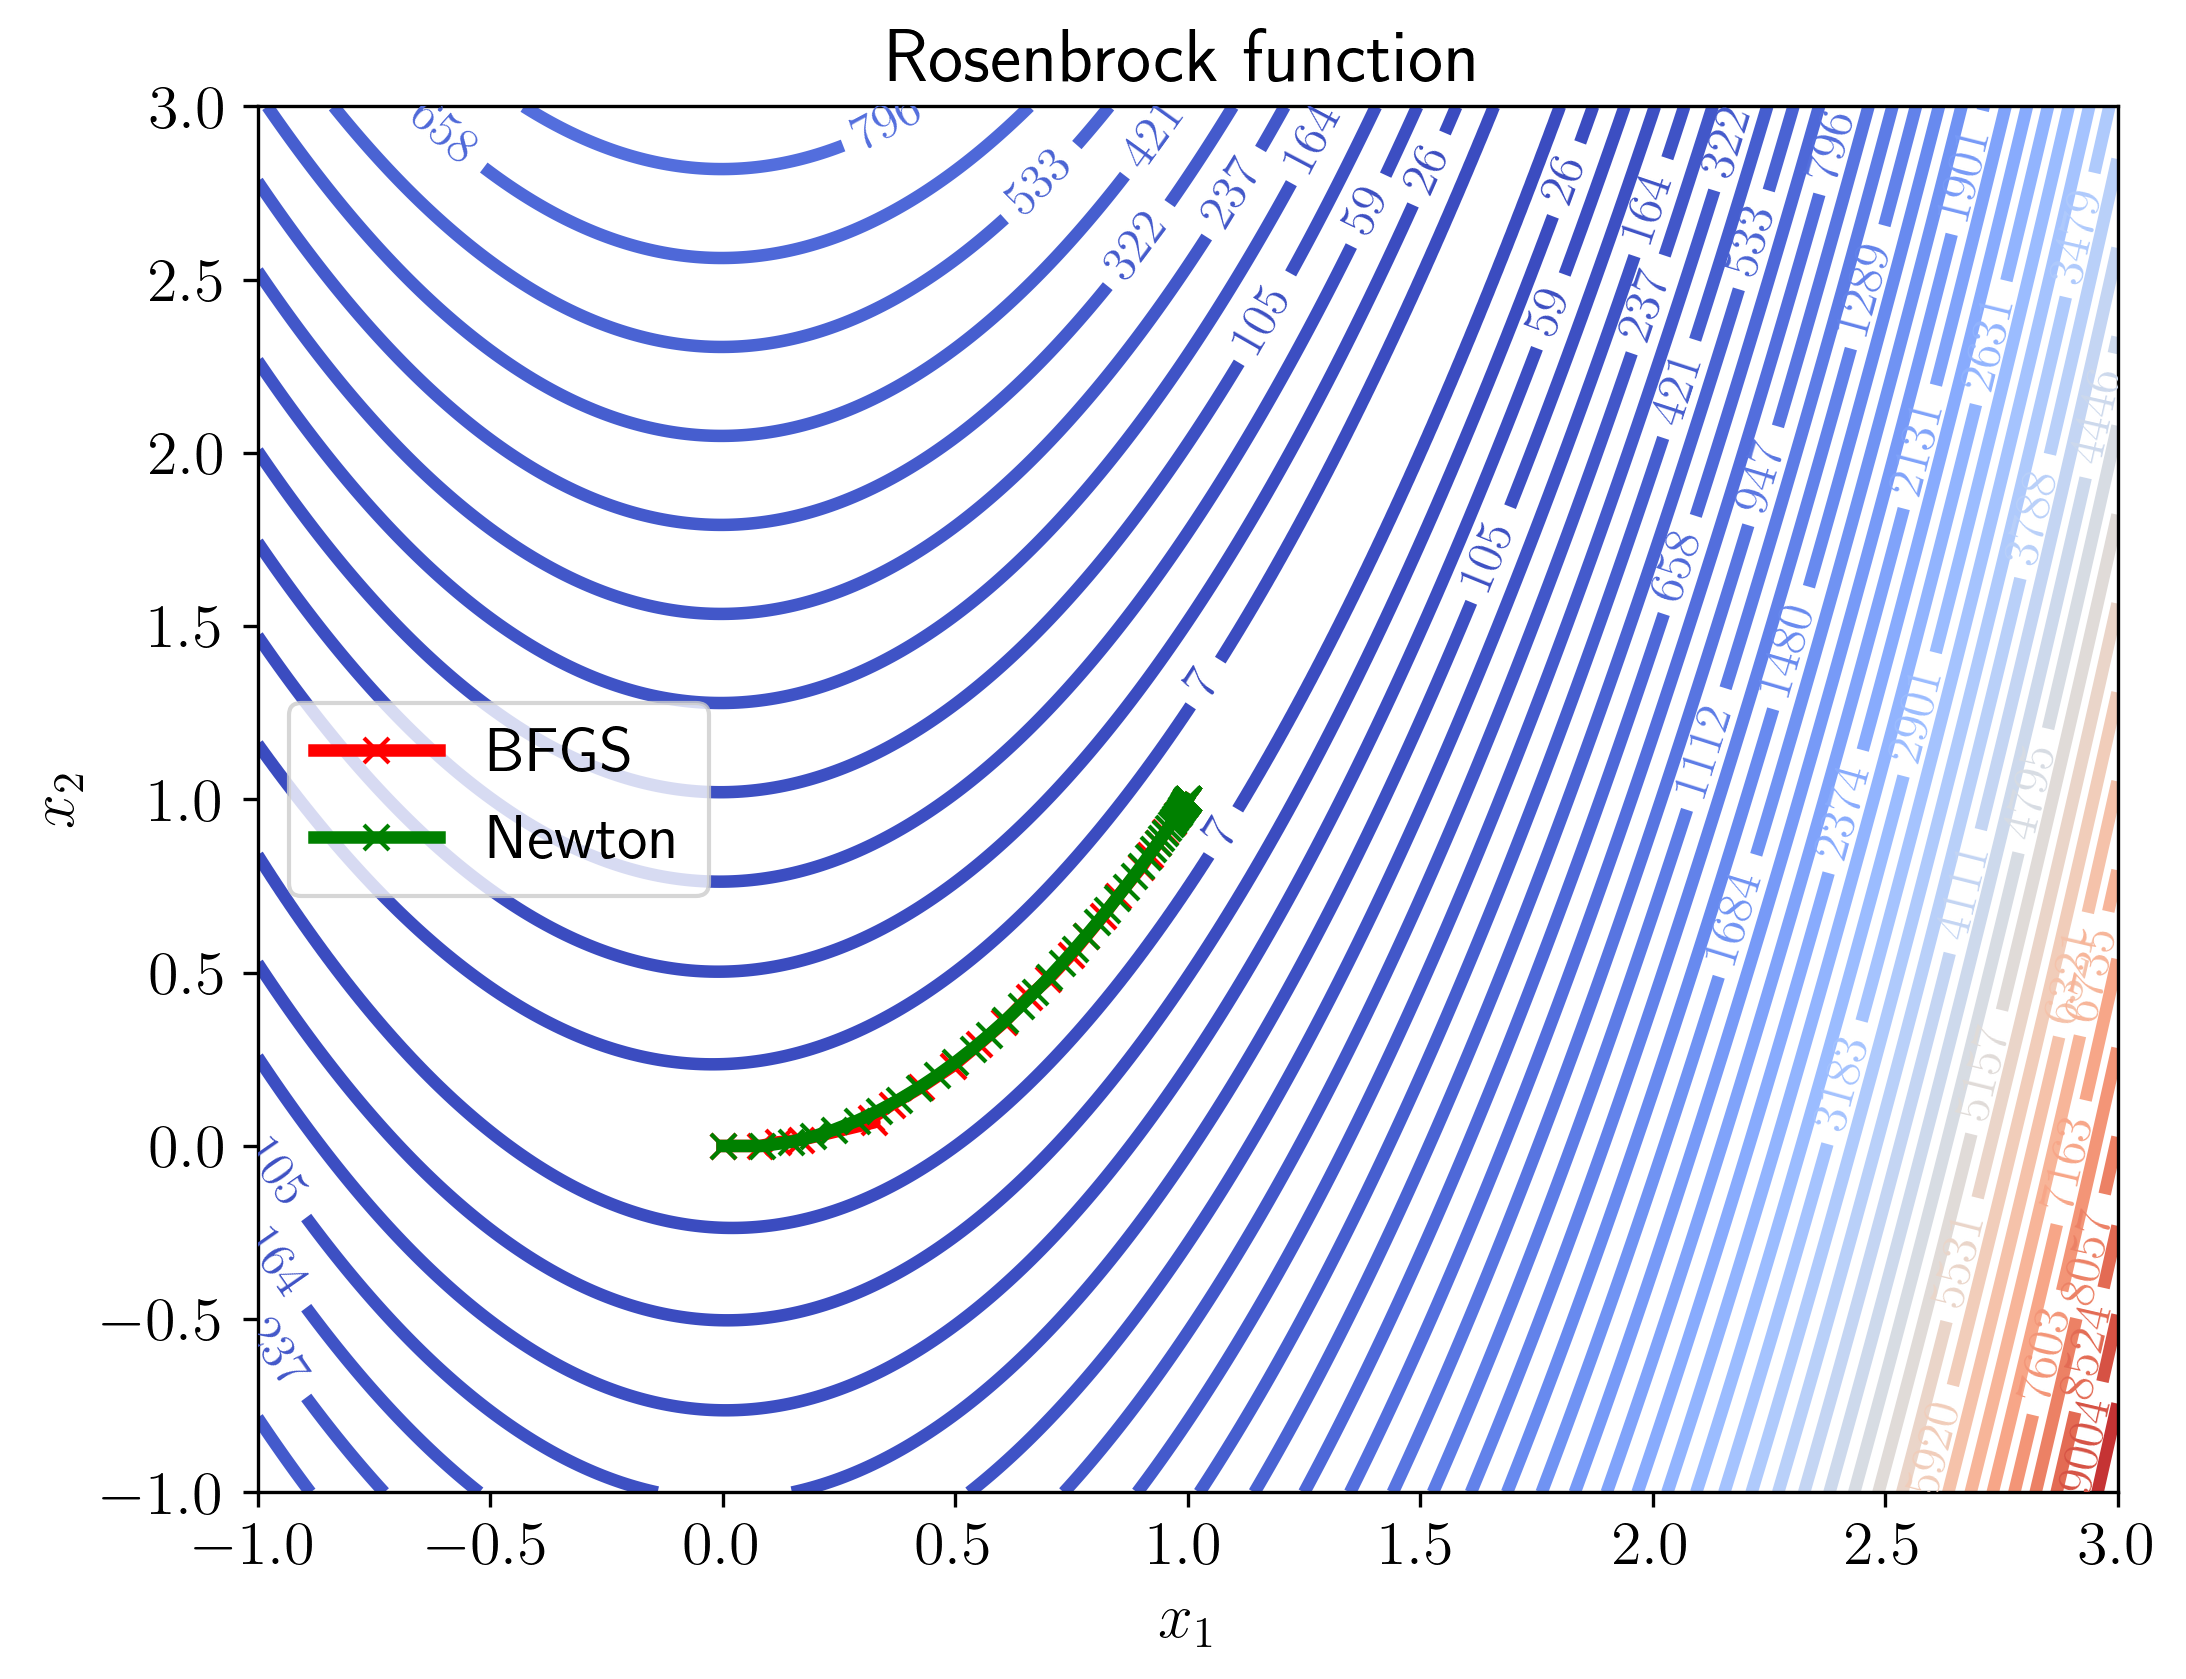
\includegraphics[width=\textwidth]{figs/rosenbrock_contour.png}
		% \caption{BFGS and Newton applied on the Rosenbrock function}
	\end{subfigure}
	\begin{subfigure}[t]{0.4\textwidth}
		\centering
		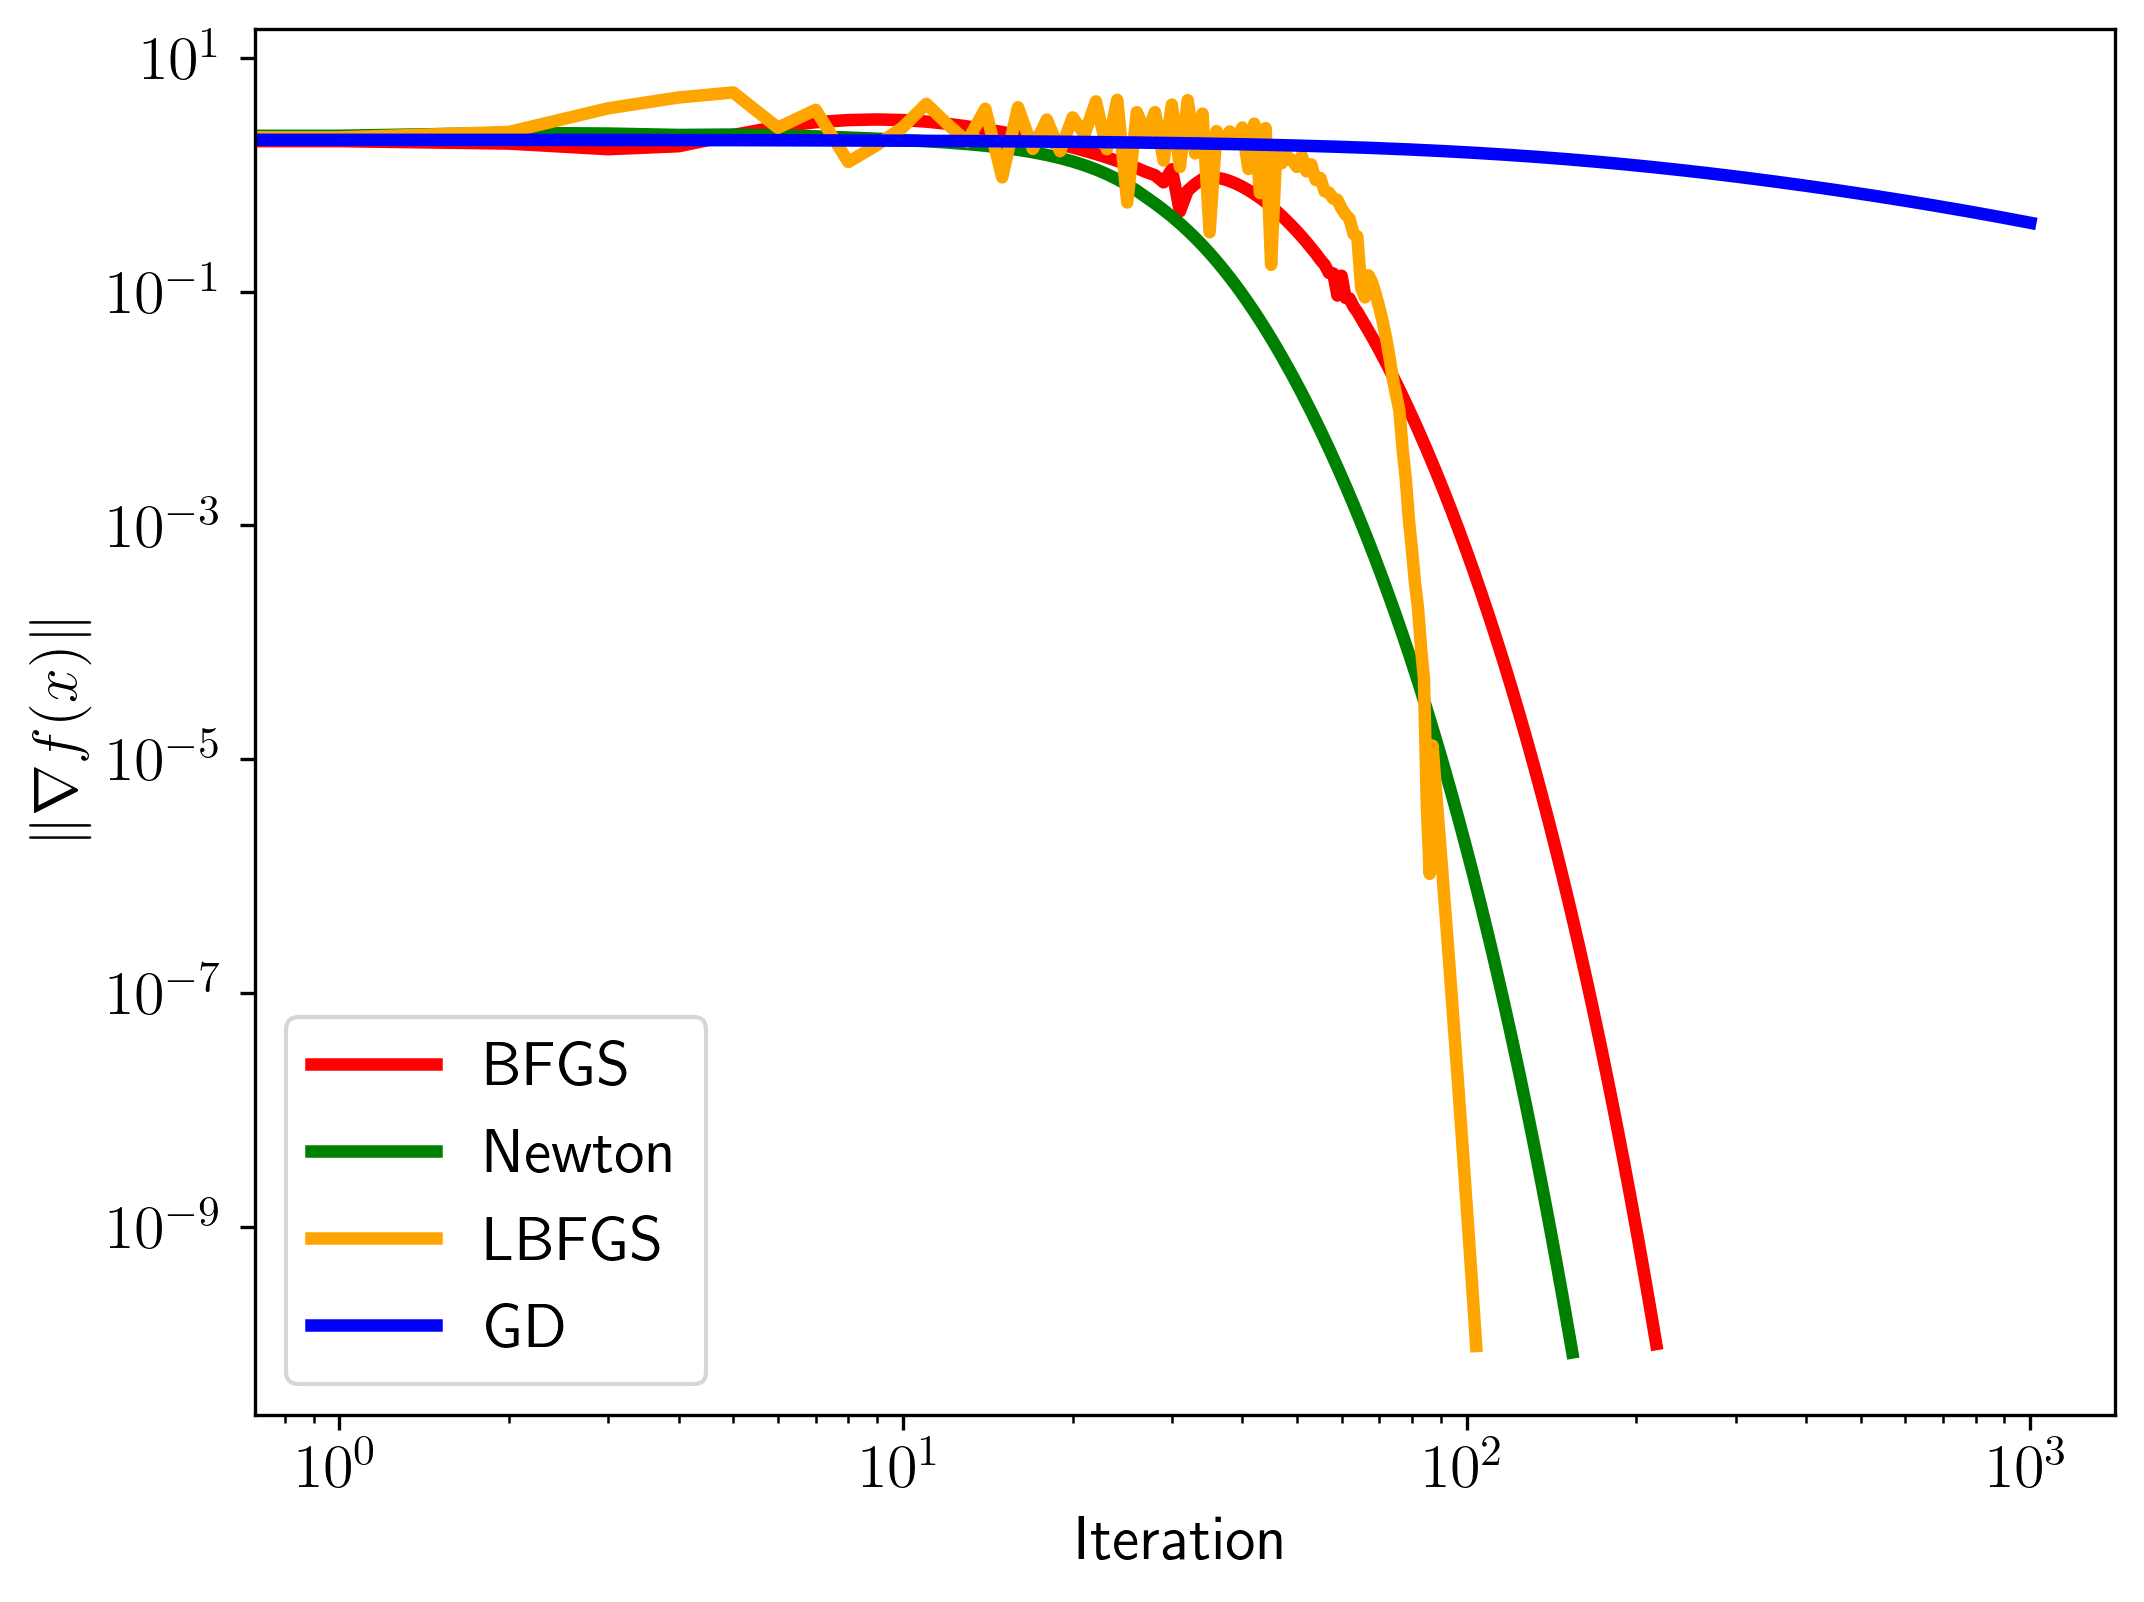
\includegraphics[width=\textwidth]{figs/rosenbrock_grad_norm_convergence.png}
		\caption{Convergence of various methods on the Rosenbrock function}
	\end{subfigure}
	\caption{BFGS and Newton applied on the Rosenbrock function}
\end{figure*}
\subsection{Comparitive study of BFGS}
Every algorithm has been given 1000 max iterations and tolerance of norm of gradient is less than 1e-6.

We compare four algorithms BFGS, Newton, L-BFGS ( A low memory variant of BFGS) and Gradient Descent (GD).
\begin{table}[htpb]
	\centering
	\caption{Final gradient norm of each method}
	\label{tab:label}
	\begin{tabular}{lllll}
		\toprule
		Function                      & BFGS                 & Newton               & LBFGS                & GD                   \\
		\midrule
		Adjiman Function(2 - D)       & nan                  & $3.72 \mathrm{e}-16$ & $5.50 \mathrm{e}-16$ & $7.70 \mathrm{e}-01$ \\
		Rosenbrock N-D(100-D)         & $9.28 \mathrm{e}-11$ & $8.52 \mathrm{e}-11$ & $9.24 \mathrm{e}-11$ & $2.92 \mathrm{e}+00$ \\
		Paviani Function(10 - D)      & nan                  & nan                  & nan                  & $8.72 \mathrm{e}-02$ \\
		Csendes Function(10 - D)      & $9.57 \mathrm{e}-11$ & $1.21 \mathrm{e}-03$ & $9.16 \mathrm{e}-11$ & $7.48 \mathrm{e}-02$ \\
		Griewank Function(2 - D)      & nan                  & $1.26 \mathrm{e}-15$ & 6.65e-11             & $8.31 \mathrm{e}-09$ \\
		Hosaki Function(2 - D)        & nan                  & $8.83 \mathrm{e}-11$ & nan                  & $8.66 \mathrm{e}-02$ \\
		Brent Function(2-D)           & $9.00 \mathrm{e}-11$ & $9.46 \mathrm{e}-11$ & $9.90 \mathrm{e}-11$ & $3.67 \mathrm{e}+00$ \\
		Giunta Function(2 - D)        & $2.22 \mathrm{e}-15$ & $1.57 \mathrm{e}-16$ & $2.67 \mathrm{e}-15$ & $1.29 \mathrm{e}-08$ \\
		Styblinski-Tang Function(2-D) & $2.93 \mathrm{e}-14$ & $0.00 \mathrm{e}+00$ & $6.39 \mathrm{e}-14$ & $9.96 \mathrm{e}-11$ \\
		Trid 6 Function(6-D)          & nan                  & $7.60 \mathrm{e}-07$ & nan                  & $4.08 \mathrm{e}+00$ \\
		\bottomrule
	\end{tabular}
\end{table}
\begin{table}[htpb]
	\centering
	\caption{Time per iteration (in seconds)}
	\label{tab:label}
	\begin{tabular}{lllll}
		\toprule
		Function                      & BFGS     & Newton  & LBFGS    & GD       \\
		\midrule
		Adjiman Function(2-D)         & 0.01741  & 0.02919 & 0.01431  & 0.004024 \\
		Rosenbrock N-D(100-D)         & 0.01578  & 0.02691 & 0.01229  & 0.003553 \\
		Paviani Function(10 - D)      & 0.4714   & 0.4163  & 0.01651  & 0.003982 \\
		Csendes Function(10 - D)      & 0.007706 & 0.06964 & 0.008144 & 0.00223  \\
		Griewank Function(2 - D)      & 0.01202  & 0.01461 & 0.01285  & 0.004034 \\
		Hosaki Function(2 - D)        & 0.02751  & 0.04954 & 0.02716  & 0.007989 \\
		Brent Function(2-D)           & 0.01732  & 0.03552 & 0.01729  & 0.005377 \\
		Giunta Function(2 - D)        & 0.01624  & 0.02645 & 0.01503  & 0.005281 \\
		Styblinski-Tang Function(2-D) & 0.01263  & 0.0217  & 0.0127   & 0.004353 \\
		Trid 6 Function(6-D)          & 0.01533  & 0.05652 & 0.01025  & 0.002685 \\
		\bottomrule
	\end{tabular}
\end{table}
\begin{table}[htpb]
	\centering
	\caption{Number of Function Evaluations}
	\label{tab:label}
	\begin{tabular}{lllll}
		\toprule
		Function                      & BFGS & Newton & LBFGS & GD   \\
		\midrule
		Adjiman Function(2 - D)       & 1426 & 956    & 1124  & 1001 \\
		Rosenbrock N-D(100 - D)       & 4744 & 2465   & 5642  & 1001 \\
		Paviani Function(10 - D)      & 1012 & 7      & 5     & 1001 \\
		Csendes Function(10 - D)      & 7826 & 169638 & 1350  & 1001 \\
		Griewank Function(2 - D)      & 2233 & 31     & 987   & 1001 \\
		Hosaki Function(2 - D)        & 2352 & 2060   & 1256  & 1001 \\
		Brent Function(2 - D)         & 2789 & 2021   & 1395  & 1001 \\
		Giunta Function(2 - D)        & 2217 & 1348   & 980   & 1001 \\
		Styblinski-Tang Function(2-D) & 2118 & 1220   & 879   & 730  \\
		Trid 6 Function(6-D)          & 2020 & 89229  & 883   & 1001 \\
		\bottomrule
	\end{tabular}
\end{table}
\begin{table}[htpb]
	\centering
	\caption{Number of Iterations}
	\label{tab:label}
	\resizebox{\columnwidth}{!}{%
		\begin{tabular}{lllll}
			\toprule
			Function                        & BFGS             & Newton           & LBFGS            & GD               \\
			\midrule
			Adjiman Function(2-D)           & Did not converge & 72               & 148              & Did not converge \\
			Rosenbrock N-D(100-D)           & 333              & 177              & 775              & Did not converge \\
			Paviani Function(10 - D)        & Did not converge & Did not converge & Did not converge & Did not converge \\
			Csendes Function(10 - D)        & 708              & Did not converge & 191              & Did not converge \\
			Griewank Function(2 - D)        & Did not converge & 6                & 138              & 1001             \\
			Hosaki Function(2 - D)          & Did not converge & 148              & Did not converge & Did not converge \\
			Brent Function(2-D)             & 199              & 145              & 200              & Did not converge \\
			Giunta Function(2 - D)          & 135              & 97               & 138              & 1001             \\
			Styblinski-Tang Function(2 - D) & 124              & 90               & 127              & 730              \\
			Trid 6 Function(6-D)            & Did not converge & 1001             & Did not converge & Did not converge \\
			\bottomrule
		\end{tabular}
	}
\end{table}

From the tables we can see that BFGS and L-BFGS converge fairly well at the cost of more function evaluations than Newton. We can se the cost per iteration is the lowest for Gradient Descent which is expected but it also didn't converge for a lot of problem whereas BFGS and L-BFGS provide a middle ground between accuracy and cost per iteration. This is especially apparent for the 100-D problem. The non convergence of BFGS in certain places is the fault of my implementation as line search might fail and there was no simple way of handling it.
% -------------------------
% Chapter 3: Conclusion
% -------------------------
\chapter{Conclusion}
The report provides introductory look at BFGS algorithm and Quasi Newton algorithms in general, including line-search theory, convergence proofs, and the inverse Hessian update derivation.  We were able to prove convergence under very restricted set of conditions, more can be said about BFGS under relaxed condition as outlined in \cite{nocedal}. We proved under the restricted conditions that BFGS is globally convergent and achieves superlinear convergence near a nondegenerate minimizer.  Numerical experiments verify our claims, it is much better than gradient descent and on par with Newton without paying for the linear system solve.

The biggest problem I encountered during this project was line search. Making a line search algorithm is quite difficult as they need to be fairly quick at finding an appropriate step size. I also had some difficulty in making my BFGS algorithm robust because there are so many ways it can go wrong from numerical instabilities to very small curvatures which make change in approximate Hessian quite big. But overall, the project was a very good experience and has definitely increased my appreciation for libraries.
% -------------------------
% Appendices
% -------------------------
\appendix


\chapter*{Appendix}
\addcontentsline{toc}{chapter}{\bf Appendix}
\renewcommand{\thesection}{\Alph{section}}

\section{Additional calculations or proof of lemmas}

\section{Pseudocode of your algorithm}

\begin{algorithm}[H]
	\caption{BFGS with Wolfe Line Search}
	\begin{algorithmic}[1]
		\State \textbf{Input:} $x_0$, $B_0=I$, tolerances $\varepsilon$
		\For{$k=0,1,2,\dots$}
		\State $p_k \gets -B_k\,\nabla f(x_k)$
		\State Find $\alpha_k$ satisfying Wolfe conditions
		\State $s_k \gets \alpha_k p_k$, \quad $y_k \gets \nabla f(x_k+s_k)-\nabla f(x_k)$
		\State Update $B_{k+1}$ via BFGS formula
		\If{$\|\nabla f(x_{k+1})\|<\varepsilon$} \textbf{break} \EndIf
		\EndFor
		\State \textbf{Output:} Approximate minimizer $x_{k+1}$
	\end{algorithmic}
\end{algorithm}
\bibliographystyle{plain}
\bibliography{refs}
\addcontentsline{toc}{chapter}{Bibliography}

\end{document}

